\documentclass[conference]{IEEEtran}

\IEEEoverridecommandlockouts
\usepackage{cite}
\usepackage{amsmath,amssymb,amsfonts}
\usepackage{graphicx}
\usepackage{textcomp}
\usepackage{xcolor}
\usepackage{booktabs}
\usepackage{multirow}
\usepackage{array}
\usepackage{url}
\usepackage{tikz}
\usepackage{listings}
\usepackage{pgfplots}
\pgfplotsset{compat=1.18}
\usetikzlibrary{positioning,arrows.meta,shapes.geometric,fit,calc,backgrounds,decorations.pathreplacing}

\definecolor{mralight}{rgb}{0.95,0.96,0.98}
\definecolor{mradark}{rgb}{0.10,0.18,0.28}
\lstset{
  basicstyle=\ttfamily\scriptsize,
  breaklines=true,
  columns=fullflexible,
  frame=single,
  framesep=4pt,
  backgroundcolor=\color{mralight},
  xleftmargin=0.4em,
  xrightmargin=0.4em,
  framextopmargin=4pt,
  framexbottommargin=4pt,
  aboveskip=1.2em,
  belowskip=1.2em
}
% Add vertical space between a top listing caption and its colored box.
\makeatletter
\let\MRA@lstMakeCaption\lst@MakeCaption
\def\lst@MakeCaption#1{\MRA@lstMakeCaption{#1}\if t#1\vskip5\p@\relax\fi}
\makeatother

\newcommand{\mra}{Marine Race Arena}
\newcommand{\cmd}[1]{\texttt{#1}}

\begin{document}

\title{\mra: A Configurable HoloOcean Benchmark for Underwater Gate Racing and Team-Level Fleet Evaluation}

\author{\IEEEauthorblockN{Lorenzo Bacchiani, Andrea Bedei, Roberto Girau and Giovanni Pau}
\IEEEauthorblockA{Department of Computer Science and Engineering, University of Bologna, Italy}
}

\maketitle

\begin{abstract}
Autonomous underwater racing lacks a reproducible benchmark that separates controller performance from privileged simulator state. We present \mra{}, a HoloOcean benchmark for autonomous underwater gate racing. The framework enforces a strict evaluation contract: controllers act only on documented onboard observations, while an independent referee uses privileged state to validate gate crossings, penalties, timeouts and scores. The architecture supports single-rover trials and cooperative multi-rover teams with independent progress tracking and team-level evaluation. A deterministic rule-based controller completed all three official clean tracks in every evaluated seed under the official observation contract. For fleet evaluation, a leader-follower controller coordinates staggered rovers through an optional acoustic channel using only legal observations and controller-authored messages. HoloOcean diagnostic validation on the clean Horseshoe Bay track confirmed the coordination under contact dynamics: all coordinated runs finished without inter-vehicle proximity events or gate/world collisions, whereas uncoordinated teams incurred repeated collisions and sometimes failed to finish. The benchmark supports reproducible evaluation of individual and cooperative control in underwater gate racing.
\end{abstract}

\begin{IEEEkeywords}
underwater robotics, autonomous racing, HoloOcean, BlueROV2, simulation benchmark, referee, multi-robot systems, team-level evaluation
\end{IEEEkeywords}

\section{Introduction}
\label{sec:introduction}

Autonomous racing has become a productive research format because it compresses perception, planning, control, and real-time decision-making into a single quantitative task under repeatable constraints~\cite{betz2022autonomous}. In ground racing, the F1TENTH platform standardizes circuits, a vehicle model, metrics, and baselines for continuous control and reinforcement learning~\cite{okelly2020f1tenth}, while full-scale leagues such as the Abu Dhabi Autonomous Racing League (A2RL) push planning and control to the limits of vehicle handling in head-to-head competition~\cite{hoffmann2026a2rl}. In aerial racing, gate-based benchmarks and competitions drove a progression from modular perception--control stacks~\cite{foehn2020alphapilot} to learning-based policies that reach champion-level performance~\cite{kaufmann2023swift}. A common thread is that a well-defined racing benchmark, with fixed geometry, an impartial referee, and machine-readable outcomes, accelerates and disciplines the comparison of autonomy methods.

Underwater robotics has mature simulation tools but lacks a comparable racing benchmark. Existing marine simulators emphasize intervention, inspection, navigation, or sensor realism rather than a compact racing protocol with explicit gates, currents, obstacles, independent scoring, and fleet evaluation. Yet underwater racing is not aerial or ground racing relocated to a different simulator. Vehicle dynamics are slow and strongly damped; global localization is unavailable and must be inferred from drifting inertial and Doppler sensing or from acoustic cues; optical perception is range-limited and degrades with turbidity; acoustic guidance is low-bandwidth and noisy; persistent currents act as a structured disturbance; and physical contact with a gate or another vehicle is ambiguous to detect. These properties change both what a controller can sense and how an evaluator must score behavior.

A benchmark for this domain must therefore separate the autonomy stack from the referee and from the simulator internals. The controller should receive only a documented \emph{official observation}---onboard sensing, an acoustic target cue, and its own race progress---while the referee may use privileged ground-truth state to decide gate crossings, collisions, timeouts, and team scoring. Without this separation, it is impossible to claim that a result was obtained under realistic information, and it is easy to inadvertently leak global pose or exact gate geometry into the control loop.

\mra{} is designed around this separation. It is neither a new hydrodynamic simulator nor a new autonomy algorithm. It is an evaluation layer built on HoloOcean~\cite{potokar2022holoocean} and a BlueROV2-class underwater vehicle~\cite{vonbenzon2022bluerov2}, in which the race---world bounds, ordered gates, start and finish, currents, obstacles, participants, sensors, and referee---is described declaratively and a controller is plugged in by implementing a small interface. The framework supports three usage categories that are kept deliberately distinct so that infrastructure claims are not confused with solved-problem claims:

\begin{itemize}
  \item \textbf{Official benchmark mode}: fixed official tracks, official gate apertures, official observation filtering that excludes ground-truth state, and reproducible referee scoring;
  \item \textbf{Diagnostic mode}: additional logs, participant-state traces, proximity diagnostics, and smoke tests used to validate the benchmark plumbing itself;
  \item \textbf{Experimental mode}: currents, obstacles, current-compensation controllers, and close-proximity fleet interaction, which are available for investigation but are \emph{not} claimed as solved v0.1 results.
\end{itemize}

The contributions of this release-candidate paper are the following.

\begin{enumerate}
  \item A declarative underwater gate-racing benchmark model: world, ordered gates with $1.5\,\text{m}\times1.5\,\text{m}$ apertures, currents, obstacles, participants, sensors, and scoring are specified in a single JSON configuration, with three official clean tracks provided.
  \item An official controller--observation contract and a HoloOcean race runner that keep ground-truth pose, simulator current vectors, and hidden gate geometry out of participant control, together with a controller interface that a custom policy satisfies by implementing three methods.
  \item An independent referee that formalizes gate-crossing geometry, missed gates, collisions, out-of-bounds and stuck conditions, timeouts, ranking, and structured event logs.
  \item A staggered fleet/team mode in which multiple BlueROV2 participants form a single team, maintain independent progress and referee state, and aggregate into one team-level score, with rover--rover proximity diagnostics.
  \item A reproducible v0.1 validation package with a deterministic rule-based baseline, clean single-rover results on three official tracks, a stable staggered two-rover demonstration, and an explicit, honest scoping of current compensation and close-proximity fleet collisions as open work.
\end{enumerate}

The remainder of the paper is organized as follows. Section~\ref{sec:related_work} reviews underwater simulators, autonomous-racing benchmarks, and multi-vehicle underwater cooperation. Section~\ref{sec:system_overview} formalizes the benchmark model and the runtime architecture. Section~\ref{sec:configuration} describes the vehicle, the HoloOcean adapter, the sensor suite, the current model, and the official observation contract. Section~\ref{sec:controller} specifies the controller interface and the baseline controllers. Section~\ref{sec:referee} formalizes gate validation, the referee state machine, and single-rover scoring. Section~\ref{sec:fleet} describes staggered fleet execution and team scoring. Section~\ref{sec:evaluation} reports the experimental evaluation. Section~\ref{sec:discussion} discusses limitations and future work, and Section~\ref{sec:conclusion} concludes.

\section{Related Work}

\subsection{Autonomous Racing as an Evaluation Paradigm}

Autonomous racing has become a useful benchmark because it compresses several hard autonomy problems into a compact, repeatable task. Vehicles must perceive the environment, estimate state, plan dynamically feasible trajectories, react to disturbances or competitors, and execute commands under strict latency constraints. The F1/10 platform was introduced as an open-source, affordable, 1/10-scale autonomous vehicle testbed with sensors, software, simulation, and competitions intended to make cyber-physical autonomy research more reproducible and accessible~\cite{okelly2019f110}. Later surveys emphasize that F1TENTH/RoboRacer has grown into a broad research ecosystem, but also that the diversity of methods can make direct comparison difficult without unified benchmark definitions and baseline results~\cite{evans2024unifyingf1tenth,charles2025roboracer}.

This history is important for underwater racing. The value of F1TENTH is not only the vehicle model; it is the combination of shared platform, software interfaces, competition rules, baselines, and metrics. Marine Race Arena follows this evaluation-centered view, but replaces the ground-track assumptions with underwater-specific elements: 3D gate traversal, depth regulation, acoustic-like guidance, marine currents, limited visibility, obstacles, and possible multi-robot interaction.

\subsection{Gate-Based Autonomous Drone Racing}

Aerial drone racing provides a second relevant model because the task is naturally gate-based and three-dimensional. The AlphaPilot system combined learned visual abstraction, nonlinear filtering, and time-optimal planning to navigate race gates during the 2019 autonomous drone racing world championship~\cite{foehn2020alphapilot}. More recent systems have demonstrated champion-level autonomous drone racing using deep reinforcement learning~\cite{kaufmann2023swift}, robust monocular perception and control in A2RL-style competition settings~\cite{bahnam2026monorace}, and pro-level racing in uninstrumented arenas~\cite{bosello2025onyourown}. Other competition reports show the importance of drift correction, gate detection, and perception-aware planning when only limited onboard sensing is allowed~\cite{azhari2025driftcorrected}.

Marine Race Arena borrows the structural idea of a gate sequence, not the vehicle dynamics or sensing assumptions. Aerial racing gates are usually crossed at high speed in air, often with lightweight cameras and IMUs. Underwater racing introduces different constraints: lower speed, stronger fluid disturbances relative to vehicle authority, depth safety, acoustic aids, light attenuation, and the possibility of evaluating ROV-like vehicles rather than only fully untethered AUVs. This motivates a benchmark format that is similar in logic but different in physical assumptions.

\subsection{Marine Robotics Simulators}

A number of underwater simulators already address the need for realistic, repeatable marine robotics development. DAVE provides an open-source underwater simulation stack with vehicles, sensors, dynamic bathymetry, ocean currents, and tools for algorithm development~\cite{zhang2022dave}. Stonefish is an open-source marine robotics simulator with advanced hydrodynamics, sensor simulation, and recent extensions supporting machine-learning research through improved sensors, tethered operations, thruster modeling, visual-light communication, and annotation tools~\cite{grimaldi2025stonefish}. UNav-Sim focuses on visually realistic underwater simulation and synthetic data generation using Unreal Engine 5~\cite{amer2023unavsim}. Recent surveys compare HoloOcean, Stonefish, DAVE, MARUS, and UNav-Sim in terms of sensor fidelity, physical modeling, task support, and sim-to-real issues~\cite{aldhaheri2025review}. HoloOcean itself has also been extended toward higher-fidelity dynamics, Unreal Engine 5 rendering, ROS~2 support, sonar improvements, semantic sensors, and environment-generation tools~\cite{romrell2025holoocean2}. 

These simulators are complementary to Marine Race Arena. They provide physics, rendering, vehicles, and sensors; Marine Race Arena provides the race-level abstraction: configured tracks, gate geometry, beacons, benchmark tasks, participant interfaces, referee state, penalties, ranking, and output logs. In other words, the proposed contribution is not another simulator backend but a benchmark and competition layer that can use such backends.

\subsection{Marine Robotics Competitions and Maritime Benchmarks}

Marine competitions have played an important role in robotics education and research. RoboSub challenges teams to build autonomous underwater vehicles capable of solving underwater mission tasks, and recent technical design reports illustrate how teams integrate vision, sonar, controls, and mechanical subsystems for the competition~\cite{denton2024oogway2023,denton2024oogway2024}. Maritime RobotX focuses primarily on autonomous surface-vessel capabilities, while related work has explored how ideas from the AI Driving Olympics and Duckietown could be adapted to RobotX using containerized agents and uniform observation/action interfaces~\cite{huang2019robotxduckietown}. MBZIRC and other field robotics challenges show the importance of autonomous multi-robot mission execution, GPS-denied navigation, and rapid deployment under real-world conditions~\cite{bhattacharya2021mbzirc}.

These competitions are valuable, but their objectives differ from underwater racing. RoboSub is mission-task oriented; RobotX is surface-vessel oriented; MBZIRC emphasizes heterogeneous aerial, ground, or maritime mission execution rather than structured underwater gate traversal. Marine Race Arena targets a narrower and more repeatable niche: underwater vehicles traversing race tracks under standardized timing and penalty rules.

\subsection{Automated Evaluation and Plug-in Agent Interfaces}

Modern autonomy benchmarks increasingly separate the evaluated agent from the evaluator. CARLA was introduced as an open urban driving simulator with configurable environments, sensors, and benchmark-style metrics~\cite{dosovitskiy2017carla}. The AI Driving Olympics used Duckietown tasks, simulators, code templates, baseline implementations, and standardized hardware to evaluate mobile-robot agents in both simulation and real settings~\cite{zilly2019aido}. Robotics extensions of OpenAI Gym further illustrate the value of common interfaces for comparing algorithms under the same virtual conditions~\cite{zamora2016gymgazebo}.

Marine Race Arena adopts the same principle. A controller is a plug-in that receives observations and returns either high-level commands or lower-level thruster commands. The referee, in contrast, is not part of the controller. It uses privileged simulator state only to score the run, validate gate passages, detect penalties, and produce logs. This separation is essential: a controller may be acoustic-only, vision-assisted, learning-based, manual, or oracle-like for debugging, but all controllers are judged by the same independent protocol.

\subsection{Positioning of Marine Race Arena}

Table~\ref{tab:related_comparison} summarizes the positioning. Existing work provides either racing platforms, gate-based aerial racing systems, underwater simulators, maritime competitions, or benchmark infrastructure. Marine Race Arena is designed to cover the specific intersection that remains weakly represented: configurable underwater racing with gate traversal, currents, obstacles, multi-robot support, independent scoring, and swappable controller plug-ins.

\begin{table*}[t]
\centering
\scriptsize
\setlength{\tabcolsep}{4pt}
\renewcommand{\arraystretch}{1.12}
\caption{Positioning of Marine Race Arena with respect to related benchmark families. The table is qualitative and emphasizes evaluation structure rather than simulator fidelity alone.}
\label{tab:related_comparison}
\begin{tabular}{p{0.20\textwidth}p{0.15\textwidth}p{0.15\textwidth}p{0.15\textwidth}p{0.25\textwidth}}
\toprule
Family & Domain & Race / gates & Swappable agents & Main limitation for this paper's target \\
\midrule
F1TENTH/RoboRacer~\cite{okelly2019f110,evans2024unifyingf1tenth,charles2025roboracer} & Ground vehicles & Yes, track racing & Yes & Ground dynamics and 2D road assumptions \\
Autonomous drone racing~\cite{foehn2020alphapilot,kaufmann2023swift,bahnam2026monorace} & Aerial vehicles & Yes, 3D gates & Usually system-specific & Air dynamics, no marine currents or underwater sensing \\
Marine simulators~\cite{zhang2022dave,grimaldi2025stonefish,amer2023unavsim,aldhaheri2025review} & Underwater / marine & Not primarily & Simulator-dependent & Provide physics and sensors, not a race referee and scoring format \\
RoboSub / RobotX / MBZIRC~\cite{denton2024oogway2023,denton2024oogway2024,huang2019robotxduckietown,bhattacharya2021mbzirc} & Marine robotics & Mission-oriented & Competition-dependent & Focus on task completion or surface vessels rather than repeatable underwater racing \\
Marine Race Arena & Underwater vehicles & Yes, configurable gate tracks & Yes & Current work is simulation-only and still requires quantitative baseline completion \\
\bottomrule
\end{tabular}
\end{table*}

\section{System Overview}

\subsection{Design Principles}

Marine Race Arena is built around four design principles.
First, the arena must be declarative: a race should be described by configuration rather than hard-coded scenario logic. Second, the autonomy stack must be replaceable: the same race should accept manual, rule-based, learning-based, acoustic-only, vision-assisted, or debugging controllers through a common interface. Third, the referee must be independent from the controller: privileged information can be used for scoring, but it must not be exposed to official controllers. Fourth, the system should remain simulator-adapter based: the benchmark layer should not depend on a single rendering or dynamics implementation.

\subsection{Architecture}

Fig.~\ref{fig:architecture} shows the high-level architecture. A race configuration defines the world bounds, gates, start pose, finish rule, beacon behavior, current profiles, obstacle generation, participants, controller selection, and referee settings. The arena builder converts this configuration into simulator objects and abstract race geometry. The simulator adapter steps the backend and returns observations. Participant controllers consume observations and output commands. The referee consumes simulator state, validates race progress, applies penalties, and writes logs and summaries.



\begin{figure*}[t]
\centering
\resizebox{0.92\textwidth}{!}{%
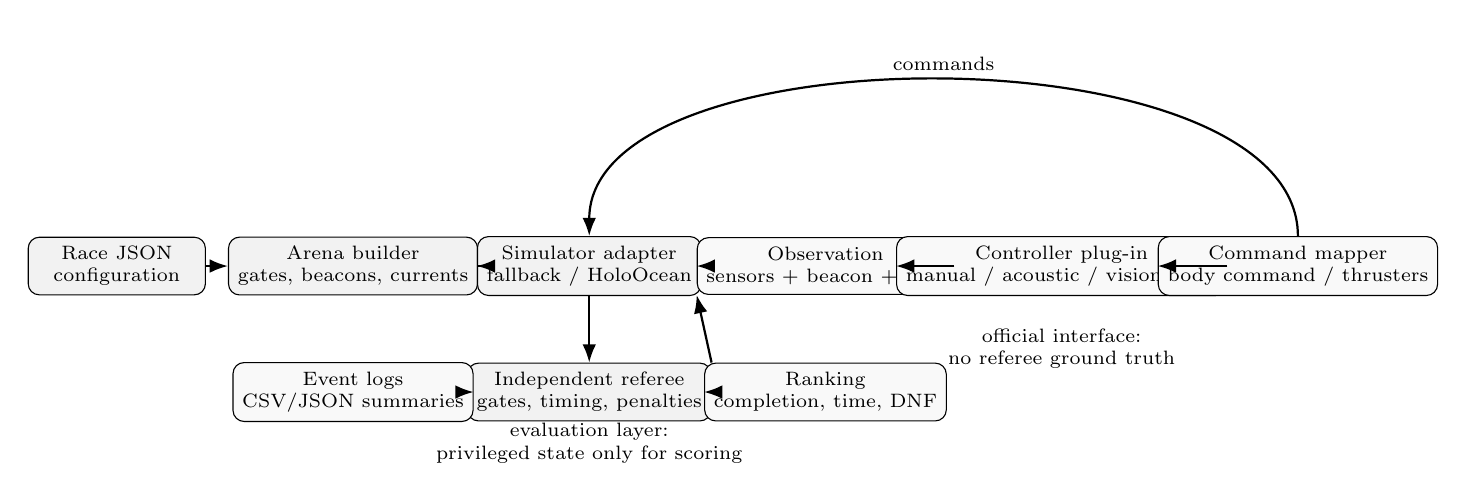
\begin{tikzpicture}[
    font=\scriptsize,
    block/.style={draw, rounded corners, align=center, minimum width=2.25cm, minimum height=0.72cm},
    arrow/.style={-Latex, thick}
]

\node[block, fill=gray!10] (config) at (0,1.8) {Race JSON\\configuration};
\node[block, fill=gray!10] (arena) at (3.0,1.8) {Arena builder\\gates, beacons, currents};
\node[block, fill=gray!10] (sim) at (6.0,1.8) {Simulator adapter\\fallback / HoloOcean};
\node[block, fill=gray!5] (obs) at (9.0,1.8) {Observation\\sensors + beacon + race};
\node[block, fill=gray!5] (ctrl) at (12.0,1.8) {Controller plug-in\\manual / acoustic / vision / RL};
\node[block, fill=gray!5] (cmd) at (15.0,1.8) {Command mapper\\body command / thrusters};

\node[block, fill=gray!10] (ref) at (6.0,0.2) {Independent referee\\gates, timing, penalties};
\node[block, fill=gray!5] (logs) at (3.0,0.2) {Event logs\\CSV/JSON summaries};
\node[block, fill=gray!5] (rank) at (9.0,0.2) {Ranking\\completion, time, DNF};

\draw[arrow] (config) -- (arena);
\draw[arrow] (arena) -- (sim);
\draw[arrow] (sim) -- (obs);
\draw[arrow] (obs) -- (ctrl);
\draw[arrow] (ctrl) -- (cmd);
\draw[arrow] (cmd.north) to[out=90,in=90,looseness=0.75] node[above]{commands} (sim.north);
\draw[arrow] (sim) -- (ref);
\draw[arrow] (ref) -- (logs);
\draw[arrow] (ref) -- (rank);
\draw[arrow] (ref.north east) -- (obs.south west);

\node[align=center] at (12.0,0.75) {official interface:\\no referee ground truth};
\node[align=center] at (6.0,-0.45) {evaluation layer:\\privileged state only for scoring};

\end{tikzpicture}}
\caption{Marine Race Arena architecture. The controller is a plug-in evaluated by an independent referee. Privileged simulator state is used for scoring and logging, but official controllers consume only allowed observations.}
\label{fig:architecture}
\end{figure*}



\subsection{Controller Interface}

The controller interface follows a simple reset-step-close lifecycle. At reset time, a controller receives race metadata. At each step, it receives an observation containing allowed sensor values, beacon information, and race progress. It returns either a high-level body-frame command, for example surge, sway, heave, and yaw, or a lower-level thruster command. This interface is intentionally small: it makes it easy to compare controllers implemented with different assumptions and different internal software stacks.

Official controllers are expected to set two semantic flags: whether they are debug-only and whether they consume ground truth. In official evaluation, debug-only or ground-truth-consuming controllers should be excluded from scientific baselines. This allows oracle controllers to remain useful for debugging tracks and referee logic without contaminating benchmark claims.

\subsection{Simulator Adapters}

The current implementation distinguishes race logic from simulator execution. A fallback adapter supports simulator-independent tests of gate validation, scoring, logging, and command flow. A HoloOcean-oriented adapter targets underwater vehicle execution in a 3D marine simulator. This separation is important because the proposed benchmark should not be tied to one version of one simulator. It also allows the referee and configuration logic to be tested without requiring graphics, hydrodynamics, or real-time rendering.

\section{Environment Design}

\subsection{Track Geometry and Gate Sequence}

A race is represented as an ordered sequence of gates. Each gate has an identifier, position, orientation, internal aperture size, bar thickness, color, and passage direction. The referee validates the abstract gate geometry rather than relying on visual collision geometry. This distinction matters because the visual bars shown in a simulator are rendering objects, whereas the scoring rule must be deterministic and independent of visual artifacts.

The current reference format uses a two-lap race over an 11-gate sequence, for 22 valid crossings in total. The gate aperture is configurable; the current marine reference configuration uses a square internal opening of $1.5\,\mathrm{m} \times 1.5\,\mathrm{m}$. The system supports single gates, double gates, vertically separated gate pairs, and split-S-like underwater sequences in which the vehicle must change depth between consecutive gates. These structures adapt the gate logic of aerial racing to slower, disturbance-prone underwater motion.

\subsection{Acoustic Beacon Guidance}

Marine Race Arena includes acoustic-beacon-like guidance associated with the next expected gate. The beacon does not validate gate passage. Instead, it provides a restricted navigation cue such as bearing, elevation, range, signal strength, update rate, and optional noise/dropout parameters. This design allows an official controller to receive useful guidance without receiving exact privileged gate geometry.

This distinction is central to the benchmark. A controller may use the beacon to approach the next gate, but it still must regulate heading, depth, and lateral alignment under vehicle dynamics and disturbances. A vision-assisted controller may combine beacon guidance with local gate observations, while an acoustic-only baseline can be evaluated as a minimal non-cheating reference.

\subsection{Marine Currents}

Currents are modeled as configurable disturbances rather than hidden implementation details. The current configuration supports profiles such as constant flow, localized jets, sinusoidal fields, and vortex-like disturbances. This enables benchmark tasks in which the same track can be evaluated under no-current, moderate-current, and structured-current conditions.

The most important design choice is that currents belong to the environment configuration, not to the controller. A benchmark run should therefore record the active current profile, random seeds, obstacle settings, and simulator adapter in its metadata. This makes later comparisons meaningful: a controller that completes a clean track cannot be compared directly with one evaluated under a localized jet unless the task definition records that difference.

\subsection{Obstacles and Arena Bounds}

The arena can include fixed or generated obstacles. Obstacles are defined with position, size, orientation, collision flag, penalty, and optionally the gate corridor in which they are placed. Generated obstacles are seeded so that obstacle-gate tasks can be repeated exactly. World bounds define legal operating space, including depth limits. Out-of-bounds events are logged and penalized according to referee settings.

The environment design therefore separates three types of geometry: abstract gate geometry for scoring, visual geometry for simulator rendering, and obstacle/bounds geometry for safety and penalties. This prevents the benchmark from depending on accidental simulator collisions for gate validation.

\section{Controller Interface and Rule Baseline}
\label{sec:controller}

A central usability goal of \mra{} is to integrate a custom autonomy stack through a small interface without modifying the runner, referee or adapter. This section specifies that interface, the dynamic loading mechanism, the action mapping and the two camera-assisted rule controllers used in the reported single-vehicle comparison.

\subsection{Controller Interface}

A controller implements three methods: \cmd{reset(mission\_info)}, called once before the run with a minimal static assignment; \cmd{step(observation)}, which receives the official observation of \eqref{eq:policy} at every control tick and returns the command of \eqref{eq:command}; and \cmd{close()}, called at teardown. The contract is duck-typed: any object exposing the three callables is accepted, so a participant need not depend on framework base classes. A manual controller may raise a dedicated stop exception from \cmd{step} to end a run cleanly; other exceptions are recorded as controller errors. Listing~\ref{lst:controller} shows a minimal example of local progression.

\begin{lstlisting}[language=Python, caption={Minimal custom controller.}, label={lst:controller}]
class MyController:
    def reset(self, mission_info):
        self.tracker = LocalCourseTracker(
            initial_beacon_id=mission_info[
                "initial_beacon_id"],
            total_beacons=mission_info[
                "total_beacons"],
            laps=mission_info["laps"])

    def step(self, observation):
        sensors = observation["sensors"]
        state = self.tracker.update(
            local_time_s=observation["local_time_s"],
            beacons=observation["beacons"],
            camera_image=sensors.get("FrontCamera"),
            dvl_velocity=sensors.get("DVLSensor"))
        if state.finished:
            return {"surge": 0.0, "sway": 0.0,
                    "heave": 0.0, "yaw": 0.0}
        # ... map state.beacon and camera to a command ...
        return {"surge": 0.3, "sway": 0.0,
                "heave": 0.0, "yaw": 0.0}

    def close(self):
        pass
\end{lstlisting}

The high-level command fields are listed in Table~\ref{tab:commands}; values are normalized to $[-1,1]$ and clamped by the framework before the action mapping. In fleet mode a controller may additionally return a small \cmd{message} payload alongside its command and read incoming teammate messages from the observation, using the optional inter-vehicle acoustic channel of Section~\ref{sec:fleet}.

\begin{table}[t]
\centering
\caption{High-level controller command fields of \eqref{eq:command}.}
\label{tab:commands}
\mratablestyle
\begin{tabular}{p{0.16\columnwidth}p{0.72\columnwidth}}
\toprule
Field & Interpretation \\
\midrule
\cmd{surge} & Longitudinal body-frame thrust; positive moves forward. \\
\cmd{sway} & Lateral body-frame thrust; sign follows the adapter mixing of \eqref{eq:thruster_mix}. \\
\cmd{heave} & Vertical thrust; additionally constrained by depth-safety logic near the bounds. \\
\cmd{yaw} & Yaw-rate command; sign follows the adapter mixing of \eqref{eq:thruster_mix}. \\
\bottomrule
\end{tabular}
\end{table}

\subsection{Dynamic Loading}

A controller is selected at run time in one of three ways: a built-in alias such as \cmd{rule\_gate\_baseline} or \cmd{rule\_gate\_center\_then\_commit}; a dotted module path with an explicit class; or a file path together with \cmd{--controller-class}, which is imported dynamically. For inspection and data collection, the runner can also be launched with the manual \cmd{keyboard} or \cmd{pygame} controllers. This lets an external policy be evaluated without modifying the package:

\begin{lstlisting}[language=bash]
python -m marine_race_arena.scripts.run_marine_race \
  --track .../marine_race_horseshoe_bay.json \
  --benchmark-task clean_gate \
  --controller path/to/my_controller.py \
  --controller-class MyController \
  --adapter holoocean --official --headless
\end{lstlisting}

\subsection{Action Mapping}

The framework clamps the returned command to $[-1,1]^4$ and applies a depth-safety rule that suppresses heave that would drive the vehicle past $z_{\min}$ or $z_{\max}$. The selected adapter then maps this portable body-frame command to its vehicle; the reference HoloOcean adapter uses \eqref{eq:thruster_mix}. That adapter may alternatively receive raw eight-thruster values, while the high-level interface remains the vehicle-independent default.

\subsection{Controller-Local Course Progression}

Both official rule controllers own a \cmd{LocalCourseTracker}; the runner supplies no progression signal. The tracker initializes from the public mission assignment \cmd{initial\_beacon\_id} and maintains a local expected beacon, completed count, lap and status through
\begin{equation*}
\begin{aligned}
\textsc{search}&\rightarrow\textsc{approach}\rightarrow\textsc{visual\_align}\\
&\rightarrow\textsc{commit}\rightarrow\textsc{verify\_exit}\rightarrow\textsc{advance},
\end{aligned}
\end{equation*}
ending in \textsc{finished} after the final locally confirmed beacon. It filters the received list for its own expected id; packets from other transmitters are not labeled or selected by the framework. Temporary visual loss, a missing packet, an isolated range jump, a range rise without a prior close approach and a commit without forward DVL displacement cannot advance the state.

The tracker enters and completes a passage only when persistent camera, acoustic and DVL evidence agrees with the expected beacon. Incomplete or inconsistent evidence returns it to local acquisition without advancing. The two reference controllers and their local-progression logic were designed and validated for the gate geometry, beacon placement, sensing configuration and vehicle dynamics of the three official circuits used in this study. After each non-final local advancement, the tracker holds an exit-clearance phase; after the final advancement, it enters \textsc{Finished} directly and commands zero. Controller-local snapshots and independent referee crossings are logged separately for offline comparison and never fed back into control.

\subsection{Rule-Based Baselines}

The two official reference controllers are deterministic and interpretable rule-based baselines rather than optimized policies. They use the same onboard inputs: received acoustic beacon packets, the forward RGB camera, depth and IMU measurements and body-frame DVL velocity. Both combine acoustic guidance, visual centering, depth hold and DVL-based passage verification through the shared \textsc{LocalCourseTracker} shown in Fig.~\ref{fig:rule_baseline_state}.

\emph{Continuous Servo} steers toward the expected beacon and uses the camera to refine alignment as the gate becomes visible. Depth feedback maintains the vertical reference, while DVL motion provides evidence that the vehicle has crossed and cleared the gate. Its defining behavior appears during \textsc{commit} and \textsc{verify\_exit}: the controller continues applying bounded visual corrections while moving through the aperture. It therefore keeps servoing toward the observed image center throughout the passage.

\begin{figure}[t]
\centering
\scriptsize
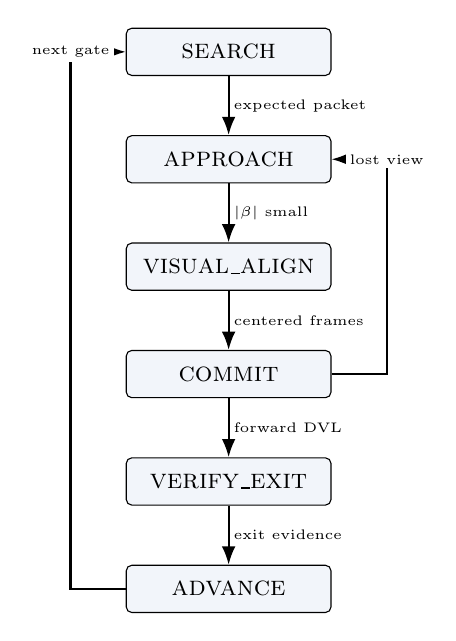
\begin{tikzpicture}[
  node distance=0.75cm,
  state/.style={draw, rounded corners=2pt, fill=mralight, align=center,
    minimum width=2.6cm, minimum height=0.6cm, inner sep=2.5pt},
  arrow/.style={-Latex, thick},
  lbl/.style={font=\tiny, fill=white, inner sep=1.5pt}
]
\node[state] (search) {\textsc{search}};
\node[state, below=of search] (approach) {\textsc{approach}};
\node[state, below=of approach] (align) {\textsc{visual\_align}};
\node[state, below=of align] (commit) {\textsc{commit}};
\node[state, below=of commit] (verify) {\textsc{verify\_exit}};
\node[state, below=of verify] (advance) {\textsc{advance}};

% forward path, straight down the centre
\draw[arrow] (search) -- node[lbl, right] {expected packet} (approach);
\draw[arrow] (approach) -- node[lbl, right] {$|\beta|$ small} (align);
\draw[arrow] (align) -- node[lbl, right] {centered frames} (commit);
\draw[arrow] (commit) -- node[lbl, right] {forward DVL} (verify);
\draw[arrow] (verify) -- node[lbl, right] {exit evidence} (advance);

% lost-view / failed-commit feedback returns to approach, routed on the right
\draw[arrow] (commit.east) -- ++(0.7,0)
  |- node[lbl, pos=0.5] {lost view} (approach.east);

% next-gate loop, routed on the left
\draw[arrow] (advance.west) -- ++(-0.7,0)
  |- node[lbl, pos=0.5] {next gate} (search.west);
\end{tikzpicture}
\caption{The \textsc{LocalCourseTracker} state machine shared by both rule controllers. \textsc{advance} loops to \textsc{search} for the next gate and reaches \textsc{finished} after the last confirmed passage.}
\label{fig:rule_baseline_state}
\end{figure}

\subsection{A Center-Then-Commit Rule Controller}
\label{sec:center_commit_baseline}

\emph{Center-then-Commit} retains the same observations, acoustic and visual guidance, shared tracker and local confirmation criterion as Continuous Servo. The only difference is the gate-passage strategy. After establishing a stable visual-acoustic lock, it stops chasing subsequent image-centroid changes during \textsc{commit} and \textsc{verify\_exit}. It instead advances through the aperture while maintaining the locked depth and attitude from onboard depth and IMU feedback; the same DVL-based evidence is used to verify the passage.

Because the observations, \textsc{LocalCourseTracker} and confirmation logic remain unchanged, the matched comparison of Section~\ref{sec:eval_comparison} isolates the effect of continuous visual correction versus a stabilized committed passage.

\begin{figure}[t]
\centering
\scriptsize
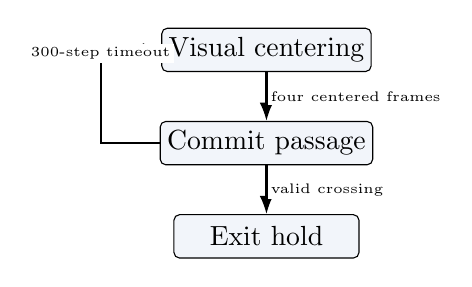
\begin{tikzpicture}[
  node distance=0.62cm,
  state/.style={draw, rounded corners=2pt, fill=mralight, align=center,
    minimum width=2.35cm, minimum height=0.55cm, inner sep=2.5pt},
  arrow/.style={-Latex, thick},
  lbl/.style={font=\tiny, fill=white, inner sep=1.2pt}
]
\node[state] (center) {Visual centering};
\node[state, below=of center] (commit) {Commit passage};
\node[state, below=of commit] (exit) {Exit hold};

\draw[arrow] (center) -- node[lbl, right] {four centered frames} (commit);
\draw[arrow] (commit) -- node[lbl, right] {valid crossing} (exit);
\draw[arrow] (commit.west) -- ++(-0.75,0)
  |- node[lbl, pos=0.48] {300-step timeout} (center.west);
\end{tikzpicture}
\caption{Center-then-commit gate passage and timeout recovery.}
\label{fig:center_commit_states}
\end{figure}




\section{Referee, Gate Validation, and Scoring}
\label{sec:referee}

The referee evaluates progress independently of the controller (requirement R3) using privileged ground-truth state. This section formalizes the gate-crossing test, the referee state machine and its arbitration order, the penalty model, and the single-rover score.

\subsection{Gate Frame and Crossing}

Each gate's orientation derives solely from its passage direction $n_g$, giving a right-handed frame
\begin{equation}
\label{eq:gate_frame}
\hat{n}=\frac{n_g}{\lVert n_g\rVert},\quad u_g=\frac{\hat{z}\times\hat{n}}{\lVert\hat{z}\times\hat{n}\rVert},\quad v_g=\hat{n}\times u_g,
\end{equation}
with world-up $\hat{z}=(0,0,1)$. For consecutive referee-side positions $p_{t-1},p_t$, the signed distances to the gate plane are
\begin{equation}
\label{eq:signed_dist}
d_{t-1}=\hat{n}^{\!\top}(p_{t-1}-c_g),\qquad d_t=\hat{n}^{\!\top}(p_t-c_g).
\end{equation}
A candidate crossing requires a sign change in the \emph{correct direction},
\begin{equation}
\label{eq:direction}
d_{t-1}\le 0\le d_t \;\wedge\; (p_t-p_{t-1})^{\!\top}\hat{n}>0,
\end{equation}
i.e.\ travel from the negative to the positive side along the normal. The intersection of the segment with the plane is
\begin{equation}
\label{eq:intersection}
\lambda=\frac{-d_{t-1}}{d_t-d_{t-1}},\quad q=p_{t-1}+\lambda\,(p_t-p_{t-1}),\quad \lambda\in[0,1],
\end{equation}
and the crossing is accepted only when $q$ lies inside the aperture, shrunk by the configured safety margin $m_g$,
\begin{equation}
\label{eq:aperture}
\big|u_g^{\!\top}(q-c_g)\big|\le \tfrac{w_g}{2}-m_g,\qquad
\big|v_g^{\!\top}(q-c_g)\big|\le \tfrac{h_g}{2}-m_g.
\end{equation}
Gates must be passed \emph{in sequence}: the referee tests only the expected gate $g_{\sigma}$, advancing the index $\sigma\!\leftarrow\!\sigma+1$ on a valid crossing and incrementing the lap when the sequence completes. A crossing of a \emph{non-target} gate aperture is a missed-gate event; a sign change in the wrong direction is logged but neither penalized nor counted as progress. Fig.~\ref{fig:gate_geometry} illustrates the test and Fig.~\ref{fig:lifecycle} the participant lifecycle.

\begin{figure}[t]
\centering
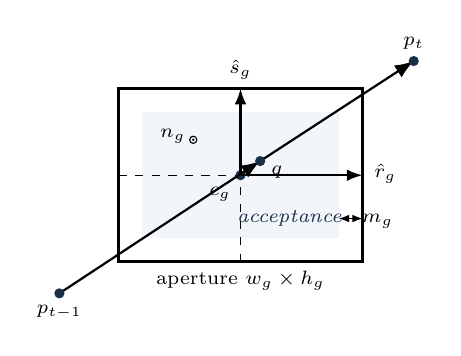
\begin{tikzpicture}[
  scale=1.0,
  font=\small,
  gate/.style={line width=1.1pt},
  axis/.style={-{Latex[length=2mm]}, thick},
  traj/.style={-{Latex[length=2.4mm]}, thick},
  dot/.style={circle, fill=mradark, inner sep=1.3pt}
]
% aperture (outer) and acceptance region (inner, shrunk by margin m_g)
\fill[mralight] (-1.25,-0.8) rectangle (1.25,0.8);
\draw[gate] (-1.55,-1.1) rectangle (1.55,1.1);
\draw[dashed] (-1.55,0) -- (1.55,0);
\draw[dashed] (0,-1.1) -- (0,1.1);
\node[font=\scriptsize] at (0,-1.34) {aperture $w_g \times h_g$};
\node[font=\scriptsize, mradark] at (0.62,-0.55) {\itshape acceptance};

% margin m_g annotation on the right edge
\draw[{Latex[length=1.3mm]}-{Latex[length=1.3mm]}] (1.25,-0.55) -- (1.55,-0.55);
\node[font=\scriptsize] at (1.74,-0.58) {$m_g$};

% gate frame at center: r_g, s_g in-plane; n_g out of plane
\node[dot] (c) at (0,0) {};
\node[font=\scriptsize] at (-0.26,-0.24) {$c_g$};
\draw[axis] (0,0) -- (1.55,0); \node[font=\scriptsize] at (1.84,0.02) {$\hat{r}_g$};
\draw[axis] (0,0) -- (0,1.1);  \node[font=\scriptsize] at (0.0,1.34) {$\hat{s}_g$};
\draw (-0.6,0.45) circle (1.3pt); \fill (-0.6,0.45) circle (0.5pt);
\node[font=\scriptsize] at (-0.86,0.5) {$n_g$};

% crossing trajectory through q
\coordinate (q) at (0.25,0.18);
\draw[traj] (-2.3,-1.5) -- (q);
\draw[traj] (q) -- (2.2,1.45);
\node[dot] at (q) {}; \node[font=\scriptsize] at (0.46,0.04) {$q$};
\node[dot] at (-2.3,-1.5) {}; \node[font=\scriptsize] at (-2.3,-1.74) {$p_{t-1}$};
\node[dot] at (2.2,1.45) {}; \node[font=\scriptsize] at (2.2,1.68) {$p_{t}$};
\end{tikzpicture}
\caption{Gate-crossing validation. A valid crossing pierces the gate plane in the normal direction (\eqref{eq:direction}) at a point $q$ (\eqref{eq:intersection}) inside the aperture shrunk on every side by the safety margin $m_g$ (\eqref{eq:aperture}); the frame $(\hat{r}_g,\hat{s}_g,n_g)$ follows the passage direction.}
\label{fig:gate_geometry}
\end{figure}

\begin{figure}[t]
\centering
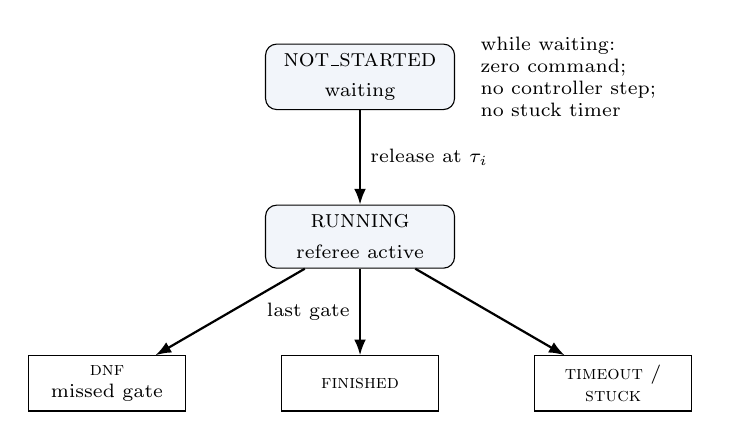
\begin{tikzpicture}[
  font=\small,
  node distance=8mm and 12mm,
  state/.style={draw, rounded corners, align=center, minimum width=24mm, minimum height=8mm, fill=mralight},
  terminal/.style={draw, align=center, minimum width=20mm, minimum height=7mm, fill=white, font=\scriptsize},
  arrow/.style={-{Latex[length=2mm]}, thick}
]
\node[state] (wait) {\textsc{not\_started}\\\scriptsize waiting};
\node[state, below=12mm of wait] (run) {\textsc{running}\\\scriptsize referee active};

\node[terminal, below=11mm of run] (finish) {\textsc{finished}};
\node[terminal, left=of finish] (dnf) {\textsc{dnf}\\\scriptsize missed gate};
\node[terminal, right=of finish] (timeout) {\textsc{timeout} /\\\textsc{stuck}};

\draw[arrow] (wait) -- node[right, font=\scriptsize]{release at $\tau_i$} (run);
\draw[arrow] (run) -- node[left, font=\scriptsize]{last gate} (finish);
\draw[arrow] (run) -- (dnf);
\draw[arrow] (run) -- (timeout);

\node[align=left, font=\scriptsize, right=2mm of wait, text width=30mm]
  {while waiting:\\ zero command;\\ no controller step;\\ no stuck timer};
\end{tikzpicture}
\caption{Participant lifecycle. A rover is released to \textsc{running} when the clock reaches its start delay $\tau_i$; before release it receives a zero command, its controller is not stepped and no stuck or gate-timeout timer accrues. Running rovers reach a terminal state by finishing the last gate, missing a gate (\textsc{dnf}) or exceeding a timeout/stuck condition. A single-rover run is the degenerate case $\tau_i=0$.}
\label{fig:lifecycle}
\end{figure}


\subsection{Referee State Machine and Arbitration}

Each participant occupies one of the states \textsc{not\_started}, \textsc{running}, \textsc{finished}, \textsc{dnf}, \textsc{timeout}, \textsc{stuck}, \textsc{manual\_stop}, or \textsc{controller\_error}; all but the first two are terminal. A participant is released to \textsc{running} when the race clock reaches its start delay (Section~\ref{sec:fleet}). On each tick of a running participant, events are evaluated in a fixed priority order that defines the arbitration: (1) a controller error transitions to \textsc{controller\_error} and returns; (2) out-of-bounds; (3) generic collision; (4) obstacle collision; (5) stuck accumulation; (6) duration timeout; (7) gate progression. Steps (2)--(5) accrue penalties without terminating; only (1), (6), a missed gate in (7), or an external gate-timeout produce a terminal state. To avoid double counting, an obstacle-collision tick suppresses the generic collision flag, and each event class has an independent cooldown.

\subsection{Penalties and Termination}

\begin{table}[t]
\centering
\caption{Referee events, their default penalty and whether they terminate the run. All values are configurable in the \texttt{referee} block; the table lists the v0.1 defaults actually applied by the referee.}
\label{tab:penalties}
\footnotesize
\renewcommand{\arraystretch}{1.2}
\begin{tabular}{p{0.34\columnwidth}p{0.20\columnwidth}p{0.30\columnwidth}}
\toprule
Event & Penalty & Terminal? \\
\midrule
Gate/bar or generic collision & $5.0$\,s each & no \\
Obstacle collision            & $5.0$\,s each\textsuperscript{\dag} & no \\
Out of bounds                 & $10.0$\,s each & no \\
Stuck (soft)                  & $15.0$\,s once & no \\
Missed gate                   & n/a            & yes (DNF) \\
Timeout (if enabled)          & n/a            & yes \\
Gate-timeout stuck (external) & n/a            & yes \\
Inter-vehicle (penalize mode) & $5.0$\,s/pair  & no (team-level) \\
\bottomrule
\end{tabular}
\par\vspace{0.6mm}
\footnotesize \textsuperscript{\dag}Per-obstacle value if specified, else the collision default. A per-event cooldown ($1.0$\,s) prevents a single sustained contact from being charged repeatedly.
\end{table}


Penalties accumulate into a per-participant total $P_i$; the defaults applied in v0.1 are listed in Table~\ref{tab:penalties}. The non-trivial conditions are formalized as follows. The instantaneous speed is $s_t=\lVert p_t-p_{t-1}\rVert/\Delta t$; a stuck accumulator integrates low-speed time,
\begin{equation}
\label{eq:stuck}
T^{\mathrm{stuck}}\!\leftarrow\!\begin{cases} T^{\mathrm{stuck}}+\Delta t, & s_t<v_{\mathrm{stuck}}\\ 0, & \text{otherwise,}\end{cases}
\end{equation}
and a one-time soft penalty is charged when $T^{\mathrm{stuck}}\ge T^{\mathrm{stuck}}_{\max}$, with $v_{\mathrm{stuck}}=0.02$\,m/s and $T^{\mathrm{stuck}}_{\max}=45$\,s. An out-of-bounds event is $p_t\notin\mathcal{B}$. A duration timeout, disabled by default, fires when $t-t_{\mathrm{green}}>T_{\max}$. A missed gate sets \textsc{dnf} when \cmd{missed\_gate\_dnf} is enabled (the default), but carries no time penalty, so a disqualifying error is never cheaper than a slow-but-legal lap.

\subsection{Single-Rover Score and Ranking}

For a finished participant the official time $T_i^{\mathrm{official}}$ is measured between the first and last gate (or green-to-finish, per the timing mode), and the score is the penalized time
\begin{equation}
\label{eq:penalized}
T_i^{\mathrm{pen}}=T_i^{\mathrm{official}}+P_i .
\end{equation}
Ranking places finished participants before unfinished ones and is defined by the ascending lexicographic key
\begin{equation}
\label{eq:ranking}
\kappa_i=\big(\,\overline{f_i},\; T_i^{\mathrm{pen}},\; -G_i,\; n_i^{\mathrm{coll}},\; P_i,\; \mathrm{dist}_i\,\big),
\end{equation}
where $\overline{f_i}=0$ for finished and $1$ otherwise, $G_i$ is the number of completed gates, $n_i^{\mathrm{coll}}$ the collision count, and $\mathrm{dist}_i$ the distance to the next gate. Thus finished rovers sort by penalized time, while unfinished rovers sort by progress, then fewer collisions, then fewer penalties, then proximity to the next gate, so partial runs remain informative rather than being discarded.

\subsection{Event Logging}

Every run emits a line-delimited event log and a machine-readable summary (requirement R5). Events include \cmd{gate\_passed}, \cmd{wrong\_direction}, \cmd{collision}, \cmd{obstacle\_collision}, \cmd{out\_of\_bounds}, \cmd{stuck}, \cmd{race\_finish}, and \cmd{dnf}, each timestamped and attributed to a participant. The summary records, per participant, the status, official and penalized times, completed gates, and counts of collisions, out-of-bounds, missed gates, and stuck events, together with the final ranking; in fleet mode it additionally carries the team summary of Section~\ref{sec:fleet}.

\section{Fleet and Team Evaluation}
\label{sec:fleet}

Fleet mode runs several vehicles as a single cooperative team through the same circuit, so the benchmark can measure how quickly the team completes the course, rather than pitting them as competitors against each other (requirement R7). The benchmark models one team only: all vehicles share a single simulated world, each controller keeps an independent local course estimate and the referee separately keeps one scoring state per vehicle. Enabling fleet mode does not alter single-vehicle behavior (R6).

\subsection{Staggered Release and Spawn Geometry}

Each participant $i$ is assigned a release delay $\tau_i=(i-1)\,\Delta\tau$ for a start gap $\Delta\tau$, so vehicles enter the course at $0,\Delta\tau,2\Delta\tau,\dots$ A waiting vehicle is sent a zero command, its controller \cmd{step} is \emph{not} called and neither stuck nor gate-timeout timers accumulate; at release the referee logs a \cmd{participant\_released} event and resets the vehicle's progress timers, so a delayed start is never misclassified as stuck or timed out. Spawn poses are laterally separated about the base spawn to reduce launch interference: using zero-based $k=0,\ldots,N-1$, the $k$-th vehicle is offset by
\begin{equation}
\label{eq:spawn_offset}
o_k = (-1)^{k}\Big\lceil \tfrac{k}{2}\Big\rceil\, s
\end{equation}
along the right axis $(-\sin\psi_0,\cos\psi_0)$ of the base yaw $\psi_0$, giving the alternating pattern $0,-s,+s,-2s,+2s,\dots$ for spacing $s$; a candidate that would fall outside the world bounds $\mathcal{B}$ is scaled inward until admissible.

\subsection{Inter-Vehicle Proximity Diagnostics}

Inter-vehicle proximity events are detected on the referee side and are never exposed to controllers. For two running vehicles $a,b$ the detector applies a separable cylinder test
\begin{equation}
\label{eq:ivc}
\sqrt{(x_a-x_b)^2+(y_a-y_b)^2}\le r_{xy}\;\wedge\;|z_a-z_b|\le r_z,
\end{equation}
with hysteresis (a pair is released only when the horizontal distance exceeds a release threshold $r_{\mathrm{rel}}$ or the vertical distance exceeds $r_z$) and a refractory cooldown to debounce sustained proximity.

\subsection{Inter-Vehicle Acoustic Communication}

Because the fleet is a single cooperative team, \mra{} provides an optional channel so that vehicles can share information while running the course. It is off by default and changes nothing for single-vehicle runs (R6). A controller transmits by returning a small \cmd{message} payload alongside its command and receives an \cmd{inbox} of teammates' messages in its observation; what a message contains and how it is used are entirely the user's responsibility, so the framework provides only the transport.

To stay faithful to the medium rather than model a perfect radio link, the channel reproduces the constraints of the underwater acoustic channel of Section~\ref{sec:related_work}. A message broadcast by vehicle $i$ reaches a teammate $j$ only if the two are within a maximum range $R_{\max}$, after a range-dependent delay
\begin{equation}
\label{eq:comms_latency}
\tau_{ij}=\frac{d_{ij}}{c}+\tau_{\mathrm{proc}},
\end{equation}
where $d_{ij}$ is the inter-vehicle distance, $c$ the speed of sound and $\tau_{\mathrm{proc}}$ a fixed processing delay; each delivery is additionally dropped with probability $p_{\mathrm{loss}}$, payloads are capped to a small size to model the low bandwidth and a vehicle may not transmit faster than a configured per-sender interval. Packet loss is drawn from a seeded generator, so a run stays reproducible.

This is an implemented acoustic-inspired transport, not a fully characterized channel model: it is the substrate for the leader-follower coordination of Section~\ref{sec:coordination} and is exercised as part of that coordination validation, but its parameters (packet loss, maximum range, latency and freshness window) are not independently swept, so we make no claim of comprehensive communication-channel validation.

\subsection{Leader-Follower Coordination}
\label{sec:coordination}

A staggered team of identical controllers stays separated in time, but a heterogeneous team does not: a faster follower released behind a slower leader catches it and they bunch up at the gates, where every vehicle converges on the same aperture center. We therefore provide a coordination controller that keeps the team a spaced convoy using only legal information and wraps a gate-passing controller that exposes a \cmd{LocalCourseTracker}, rather than replacing it, so coordination and gate navigation stay separable. Both official camera-assisted controllers satisfy this interface.

The controller is a thin, fully distributed layer over the acoustic channel of \eqref{eq:comms_latency}. Each vehicle is assigned a predecessor from the static release order in its legal mission information; the frontmost vehicle has no predecessor and races freely. Within the channel's transmit-rate limit, every vehicle periodically broadcasts exactly the three fields \cmd{local\_beacon\_index}, \cmd{local\_lap} and \cmd{local\_status}, read from its own base controller's \cmd{LocalCourseTracker}. The receiver treats these fields as estimates, retains the most recently received predecessor report and ignores it after a $2.5$\,s freshness window. Let $\hat g_i$ denote cumulative locally estimated progress reconstructed from the reported lap and beacon index. A follower yields while its predecessor is fewer than $\Delta g$ locally estimated gates ahead,
\begin{equation}
\label{eq:yield}
\text{yield}_j \iff \hat g_{\mathrm{pred}(j)}-\hat g_j<\Delta g ,
\end{equation}
and otherwise it runs its wrapped base controller unchanged. While yielding, the wrapper still updates the base tracker from onboard observations but commands zero motion. This deliberate wait can therefore trigger the independent stuck penalty and remains visible in the result. A predecessor locally reported as finished, a missing report or a report older than the freshness window stops blocking. With the channel disabled no report is delivered and the wrapper reduces to the uncoordinated base behavior.

The design turns controller-local progress estimates into physical separation. Because the gates are ordered and spatially separated, a one-gate estimated lead ($\Delta g=1$) already holds the follower one gate behind its predecessor, and a two-gate lead ($\Delta g=2$) is a more conservative margin that retains an extra intervening gate. In the coordination validation of Section~\ref{sec:eval_holoocean_coord}, $\Delta g=1$ finishes every run with no gate, world, proximity, out-of-bounds or stuck event and is faster than $\Delta g=2$; it is therefore the recommended default, with $\Delta g=2$ retained as a conservative comparison. The policy reads only the official observation, its own tracker, the static predecessor assignment and controller-authored messages; referee progress can disagree with either local estimate but never changes a coordination decision.

\subsection{Team-Level Score}

Only the \cmd{team\_summary} is the official fleet result; per-vehicle rows are diagnostics. For a team $\mathcal{P}$ of $N$ vehicles with $G_{\mathrm{exp}}$ expected gates each,
\begin{equation}
\label{eq:team_gates}
G_{\mathrm{team}}^{\mathrm{exp}}=N\,G_{\mathrm{exp}},\qquad
G_{\mathrm{team}}^{\mathrm{done}}=\sum_{i\in\mathcal{P}} G_i^{\mathrm{done}}.
\end{equation}
The team finishes only if every vehicle finishes,
\begin{equation}
\label{eq:team_finished}
\mathrm{finished}_{\mathrm{team}}=\bigwedge_{i\in\mathcal{P}}\mathrm{finished}_i,
\end{equation}
in which case the team elapsed time spans the first release to the last finish,
\begin{equation}
\label{eq:team_time}
T_{\mathrm{team}}=\max_{i} T_i^{\mathrm{finish}}-\min_{i} T_i^{\mathrm{release}},
\end{equation}
and the penalized team score aggregates every per-vehicle penalty together with the team-level inter-vehicle term,
\begin{equation}
\label{eq:team_pen}
T_{\mathrm{team}}^{\mathrm{pen}}=T_{\mathrm{team}}+\sum_{i\in\mathcal{P}} P_i+P_{\mathrm{ivc}},
\end{equation}
where $P_i$ is the per-vehicle penalty total of \eqref{eq:penalized} and $P_{\mathrm{ivc}}$ counts each inter-vehicle proximity event once per pair, not once per vehicle. Fig.~\ref{fig:fleet_scoring} illustrates the aggregation.

\begin{figure}[t]
\centering
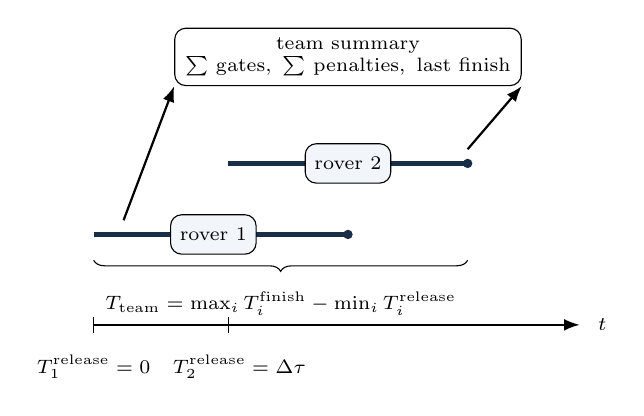
\begin{tikzpicture}[
  x=0.95cm, y=0.82cm, font=\small,
  arrow/.style={-{Latex[length=2mm]}, thick},
  rover/.style={draw, rounded corners, align=center, fill=mralight, minimum height=5mm, font=\scriptsize},
  bar/.style={line width=2pt, mradark}
]
% team summary box (top)
\node[draw, rounded corners, align=center, fill=white, minimum width=44mm, font=\scriptsize]
     (team) at (3.4,4.15) {team summary\\ $\textstyle\sum$ gates,\, $\textstyle\sum$ penalties,\, last finish};

% rover activity bars (release -> finish)
\draw[bar] (1.8,2.5) -- (5.0,2.5);
\node[rover] at (3.4,2.5) {rover 2};
\node[circle, fill=mradark, inner sep=1.2pt] at (5.0,2.5) {};

\draw[bar] (0,1.4) -- (3.4,1.4);
\node[rover] at (1.6,1.4) {rover 1};
\node[circle, fill=mradark, inner sep=1.2pt] at (3.4,1.4) {};

% contributions to the team summary (routed to avoid crossing the bars)
\draw[arrow] (0.4,1.62) -- (team.south west);
\draw[arrow] (5.0,2.72) -- (team.south east);

% team elapsed-time bracket: earliest release -> latest finish
\draw[decorate,decoration={brace,amplitude=4pt,mirror}] (0,1.0) -- (5.0,1.0);
\node[font=\scriptsize, anchor=north] at (2.5,0.66)
     {$T_{\mathrm{team}}=\max_i T_i^{\mathrm{finish}}-\min_i T_i^{\mathrm{release}}$};

% time axis with release ticks
\draw[arrow] (0,0) -- (6.5,0);
\node[font=\scriptsize] at (6.8,0) {$t$};
\foreach \x/\lab in {0/{$T_1^{\mathrm{release}}=0$}, 1.8/{$T_2^{\mathrm{release}}=\Delta\tau$}} {
  \draw (\x,0.12) -- (\x,-0.12);
}
\node[font=\scriptsize, anchor=north] at (0,-0.32) {$T_1^{\mathrm{release}}=0$};
\node[font=\scriptsize, anchor=north] at (1.95,-0.32) {$T_2^{\mathrm{release}}=\Delta\tau$};
\end{tikzpicture}
\caption{Team-level scoring for a staggered two-rover fleet.}
\label{fig:fleet_scoring}
\end{figure}


\section{Experimental Evaluation}
\label{sec:evaluation}

This evaluation does not seek an optimal underwater racing controller. It tests whether the benchmark, official observation contract, referee and team scoring behave as specified. It also reports where the reference baseline fails.

\subsection{Protocol and Metrics}

The evaluation has three experiment groups. First, the HoloOcean clean/current validation covers the three official clean tracks, the two-rover smoke demonstration on Horseshoe Bay and the \texttt{medium} and \texttt{strong} current profiles on Horseshoe Bay. These experiments use the HoloOcean adapter with the BlueROV2 agent, a control timestep of $\Delta t=0.033$\,s, official mode and the unmodified official gate apertures (requirement R4). Because HoloOcean execution is not bit-deterministic, each condition in Table~\ref{tab:validation_results} is evaluated over five seeds.

Second, the deterministic fallback controller/fleet comparison uses the deterministic kinematic adapter on Horseshoe Bay in official mode. It compares two single-rover controllers and three-, four- and five-rover fleets with and without leader-follower coordination. These results are exactly reproducible. Inter-vehicle proximity events on this substrate represent geometric proximity, not contact dynamics.

Third, the HoloOcean diagnostic validation of coordination returns to the HoloOcean adapter. Its scope is only the clean Horseshoe Bay track with three rovers, no currents or obstacles, two start gaps ($8.0$ and $0.0$\,s) and three seeds. It compares the same team with and without leader-follower coordination in diagnostic inter-vehicle mode.

The HoloOcean clean/current metrics are course completion, completed gates, official time, penalized time from \eqref{eq:penalized}, gate/world collisions, out-of-bounds events and stuck events. The deterministic comparison also reports command smoothness, inter-vehicle proximity events and team penalized time. The HoloOcean diagnostic validation of coordination reports team completion, inter-vehicle proximity events, gate/world collisions and team times. Completed-gate and gate/world collision statistics include all seeds. Time statistics include finished runs only and are omitted when no seed finishes.

\subsection{Single-Rover Clean Tracks}
\label{sec:eval_clean}

\begin{table*}[t]
\centering
\caption{Final HoloOcean clean-track, current and homogeneous two-rover fleet results over five seeds per case.}
\label{tab:validation_results}
\mratablestyle
\begin{tabular}{llrlrrr}
\toprule
Setting & Controller and track & Seeds & Status & Gates & Time (s) & Collisions \\
\midrule
\multirow{6}{*}{Clean}
 & Continuous servo, Horseshoe Bay & 5 & 5/5 FIN & 12.0/12 & $194.5\pm4.3$ & 0.0 \\
 & Center-then-commit, Horseshoe Bay & 5 & 5/5 FIN & 12.0/12 & $197.7\pm6.3$ & 0.0 \\
 & Continuous servo, Vertical Serpent & 5 & 5/5 FIN & 17.0/17 & $236.9\pm5.7$ & 0.0 \\
 & Center-then-commit, Vertical Serpent & 5 & 4/5 FIN & 14.8/17 & $241.1\pm1.6$ & 0.0 \\
 & Continuous servo, Mixed Endurance & 5 & 2/5 FIN & 17.0/22 & $394.7\pm2.8$ & 0.0 \\
 & Center-then-commit, Mixed Endurance & 5 & 5/5 FIN & 22.0/22 & $410.7\pm7.9$ & 0.0 \\
\midrule
\multirow{4}{*}{Currents}
 & Continuous servo, Horseshoe medium & 5 & 2/5 FIN & 8.4/12 & $337.9\pm13.6$ & 43.4 \\
 & Center-then-commit, Horseshoe medium & 5 & 3/5 FIN & 8.8/12 & $217.3\pm1.2$ & 25.2 \\
 & Continuous servo, Horseshoe strong & 5 & 0/5 FIN & 3.0/12 & \textemdash & 0.0 \\
 & Center-then-commit, Horseshoe strong & 5 & 0/5 FIN & 3.2/12 & \textemdash & 0.8 \\
\midrule
\multirow{2}{*}{Fleet, gap 90 s}
 & Continuous servo, team aggregate & 5 & 5/5 FIN & 24.0/24 & $303.1\pm2.9$ & 0.0 \\
 & Center-then-commit, team aggregate & 5 & 5/5 FIN & 24.0/24 & $308.0\pm5.2$ & 0.0 \\
\bottomrule
\end{tabular}
\mratablenote Times are mean$\pm$population standard deviation over finished runs. Gates and collisions are five-seed means; fleet values are team-level and collisions combine gate and world events. Medium-current penalized times are $692.9\pm53.6$\,s for continuous servo and $223.9\pm1.5$\,s for center-then-commit.
\end{table*}


Table~\ref{tab:validation_results} reports the clean-track results over five seeds. The official rule baseline completes all three courses in every seed: $12/12$, $17/17$ and $22/22$ gates, or 100\% completion. No run records an out-of-bounds or stuck event. Mean gate/world collisions remain below one per run: $0.6\pm0.5$, $0.2\pm0.4$ and $0.8\pm0.8$ on Horseshoe Bay, Vertical Serpent and Mixed Endurance. Official times are stable across seeds at $232.4\pm7.5$\,s, $259.7\pm27.8$\,s and $540.6\pm7.7$\,s. These results establish that the official clean tasks are feasible and reproducible under the official observation contract.

\subsection{Staggered Fleet and Team Scoring}

The bottom block of Table~\ref{tab:validation_results} reports the stable two-rover staggered demonstration on Horseshoe Bay over five seeds. Both rovers finish $12/12$ gates in every seed. The first rover finishes in $230.7\pm5.4$\,s with $1.4\pm0.5$ gate/world collisions. The second finishes in $236.5\pm1.4$\,s with $1.2\pm0.4$ gate/world collisions. The team completes $24/24$ gates in every seed. Its elapsed time is $340.7\pm1.4$\,s from first release to last finish, and its penalized time is $353.7\pm3.2$\,s. No inter-vehicle proximity events are recorded because the $90$\,s start gap deliberately separates the rovers. The run therefore tests multi-rover spawning, staggered release, independent per-rover referee state, ranking and team aggregation without physical interaction. It is a low-contact smoke demonstration of the fleet and team machinery.

\subsection{Behavior Under Currents}
\label{sec:eval_currents}

Clean-track performance degrades as current strength increases. On Horseshoe Bay, the rule baseline finishes only $3/5$ seeds under the \texttt{medium} profile. Across all five seeds, it completes $10.8\pm1.5$ of $12$ gates and accumulates $82.6\pm74.1$ gate/world collisions. Among the three finished seeds, official time is $315.0\pm42.3$\,s and penalized time is $428.3\pm98.5$\,s. Under the \texttt{strong} profile, the baseline never finishes. Every seed reaches only $3/12$ gates within the time limit and accumulates $11.0\pm1.1$ gate/world collisions. These results quantify the degradation under the official observation contract with the gates, margins and current profiles unchanged (requirement R4). Designing controllers that reject the current remains future work (Section~\ref{sec:discussion}).

\subsection{Controller Comparison and Fleet Coordination}
\label{sec:eval_comparison}

This experiment asks whether the benchmark separates controllers and whether coordination controls fleet interaction. It uses the engine-free deterministic kinematic adapter on Horseshoe Bay in official mode. The official gate apertures, referee rules and inter-vehicle thresholds remain unchanged (R4). The results are exactly reproducible and isolate the control logic. Inter-vehicle proximity events represent geometric proximity on this substrate, not HoloOcean contact dynamics.

The two controllers occupy different operating points. Both finish all $12$ gates. \cmd{acoustic\_baseline} takes $120.1$\,s, whereas the conservative \cmd{smooth\_gate\_baseline} takes $198.0$\,s, or $1.6\times$ as long. The mean per-step change in surge and yaw commands is used as a lower-is-smoother proxy. It drops from $0.0159$ to $0.0035$, a reduction of roughly $4.5\times$. The benchmark therefore distinguishes the two legal controllers by completion time and behavior.

The fleet comparison uses a slower \cmd{smooth\_gate\_baseline} leader with faster \cmd{acoustic\_baseline} followers. The start gap is $8$\,s, lateral spacing is $1.5$\,m and scoring uses \cmd{penalize} mode. Without coordination, the followers overtake the leader and trigger the proximity detector. Teams of three, four and five record $2$, $3$ and $4$ inter-vehicle proximity events, respectively (Table~\ref{tab:coordination}). Leader-follower coordination removes all of these events, matching the single-rover result, while every rover finishes the full gate sequence. Team time increases because the followers pace behind the leader instead of overtaking it. This is the measured safety-throughput tradeoff.

\begin{table}[t]
\centering
\caption{Fleet coordination on the deterministic kinematic substrate (Horseshoe Bay, official mode, penalize mode for inter-vehicle proximity events). A staggered heterogeneous team has a slower \texttt{smooth\_gate\_baseline} leader and faster \texttt{acoustic\_baseline} followers. Each team size is run with and without leader-follower coordination. Every rover finishes in every condition.}
\label{tab:coordination}
\footnotesize
\setlength{\tabcolsep}{5pt}
\renewcommand{\arraystretch}{1.15}
\begin{tabular}{rlrr}
\toprule
Team & Condition & Inter-vehicle $\downarrow$ & Team penalized (s) \\
\midrule
\multirow{2}{*}{3} & no coordination & 2 & 216.1 \\
 & leader-follower & \textbf{0} & 251.1 \\
\midrule
\multirow{2}{*}{4} & no coordination & 3 & 221.9 \\
 & leader-follower & \textbf{0} & 274.1 \\
\midrule
\multirow{2}{*}{5} & no coordination & 4 & 226.8 \\
 & leader-follower & \textbf{0} & 295.5 \\
\bottomrule
\end{tabular}
\end{table}


The two-gate yield margin of \eqref{eq:yield} is necessary. With a one-gate margin ($\Delta g=1$), a follower can reach a gate just as its predecessor clears it, so a full gate of physical spacing is not preserved. The four-rover team then records $6$ inter-vehicle proximity events, twice the uncoordinated team's $3$. With $\Delta g=2$, it records none. The coordination also tolerates channel loss. Repeating the four-rover coordinated run with $20\%$ per-link packet loss still yields no inter-vehicle proximity events and every rover finishes. Periodic heartbeats and the freshness window absorb the dropped packets. These results support the separation argument of Section~\ref{sec:coordination}: a two-gate progress lead becomes physical spacing. The deterministic kinematic substrate isolates this proximity logic but does not model contact. The next subsection tests the same policy in HoloOcean.

\subsection{HoloOcean Diagnostic Validation}
\label{sec:eval_holoocean_coord}

HoloOcean diagnostic validation tests the same coordination under contact dynamics. It uses only the clean Horseshoe Bay track in official mode with three rovers, no currents or obstacles, two start gaps ($8.0$ and $0.0$\,s) and three seeds. The team has a \cmd{smooth\_gate\_baseline} leader and \cmd{acoustic\_baseline} followers. Inter-vehicle mode is diagnostic and no parameters are retuned. All six coordinated runs finish with $36/36$ team gates. They record no inter-vehicle proximity events, gate/world collisions, out-of-bounds events or stuck events. Penalized time ranges from $130.7$--$131.3$\,s (Table~\ref{tab:holoocean_coordination}). Without coordination, faster followers crowd the slower leader. These runs record one or two inter-vehicle proximity events and up to $531$ gate/world collisions. In two of the six runs, both with the $8$\,s gap, the leader remains unfinished at $4/12$ gates.

Contact dynamics change the tradeoff observed on the deterministic kinematic substrate. There, coordination removes inter-vehicle proximity events at a small time cost. In HoloOcean, the same crowding produces costly gate/world collisions, so coordination becomes a net gain. Finished uncoordinated runs are slightly faster in raw time ($104$--$118$\,s versus $\sim\!131$\,s when coordinated). Once gate/world collisions are scored, their penalized times rise to $222$--$404$\,s. Two of the six uncoordinated runs do not finish. This HoloOcean diagnostic validation is deliberately limited to one clean track, three rovers, two start gaps and three seeds. Extending it to other tracks, currents, obstacles and larger fleets remains future work (Section~\ref{sec:discussion}).

\begin{table*}[t]
\centering
\caption{Three-vehicle coordination on clean Horseshoe Bay over three seeds per condition.}
\label{tab:holoocean_coordination}
\mratablestyle
\begin{tabular}{llrlrrr}
\toprule
Setting & Policy & Seeds & Status & Gates $\uparrow$ & Team time (s) $\downarrow$ & Events $\downarrow$ \\
\midrule
\multirow{3}{*}{Gap 0 s}
 & No coordination & 3 & 3/3 FIN & 36.0/36 & $219.7\pm2.5$ & 9.3 / 2.3 / 0.0 \\
 & LF(1) & 3 & 3/3 FIN & 36.0/36 & $262.3\pm7.7$ & 0.0 / 0.0 / 0.0 \\
 & LF(2) & 3 & 3/3 FIN & 36.0/36 & $288.3\pm1.3$ & 0.0 / 0.0 / 1.0 \\
\midrule
\multirow{3}{*}{Gap 8 s}
 & No coordination & 3 & 2/3 FIN & 34.3/36 & $254.0\pm24.5$ & 127.3 / 2.0 / 0.0 \\
 & LF(1) & 3 & 3/3 FIN & 36.0/36 & $266.0\pm8.3$ & 0.0 / 0.0 / 0.0 \\
 & LF(2) & 3 & 3/3 FIN & 36.0/36 & $285.7\pm3.8$ & 0.0 / 0.0 / 0.0 \\
\bottomrule
\end{tabular}
\mratablenote Times are raw team elapsed mean$\pm$sample standard deviation over full-team finishes; gates and events are three-seed means. Events are GW / IV / S: gate and world collisions, inter-vehicle proximity and stuck. No run records an out-of-bounds event. Penalized time differs for no coordination at gaps 0 and 8 s ($266.4\pm64.1$ and $564.0\pm463.0$\,s) and LF(2) at gap 0 s ($303.3\pm1.3$\,s).
\end{table*}


\subsection{Reproducibility}

Every run emits a structured event log and summary. The repository provides the exact commands used here~\cite{holodronecompetition2026}. A single configuration-driven entry point and per-track JSON files make each official run reproducible from one command. The fleet demonstration and unit-test suite are also scripted, so Table~\ref{tab:validation_results} can be regenerated end to end. One engine-free command produces the deterministic comparison in Table~\ref{tab:coordination} bit-for-bit.

\section{Discussion, Limitations and Future Work}
\label{sec:discussion}

The experiments show that completion depends on both course structure and environmental conditions: the two reference controllers clear the short clean circuit but separate on the longer track and under current, and success on clean tracks does not imply robustness to disturbances. The coordination study shows that a fully distributed leader-follower layer, using only legal onboard estimates and an acoustic-inspired channel, removes the physical interaction that an uncoordinated heterogeneous convoy suffers, with the one-gate margin doing so at the lowest time cost. Throughout, controller-local progression and independent referee scoring are kept separate, and their occasional disagreement is logged rather than reconciled, which is what lets the same contract score arbitrary controllers.

\subsection{Limitations}
\label{sec:limitations}

The evaluation is deliberately scoped, and several boundaries should be read with the results. The quantitative current sweep is limited to Horseshoe Bay; the medium and strong profiles are available on all three circuits but only Horseshoe Bay is measured. The coordination validation is limited to one clean track, three vehicles, two start gaps and three seeds. Both reference controllers are rule-based and interpretable rather than optimized, and no learning-based controller is reported. All results are in simulation: no real underwater-vehicle experiment is included, and the numbers depend on the HoloOcean vehicle and sensor models. The inter-vehicle acoustic channel is exercised only as the substrate for coordination; its packet-loss, range, latency and freshness parameters are not independently characterized. The strong-current condition acts primarily as a saturation regime that limits forward progress rather than a controllable disturbance. Finally, the two-parameter beacon-noise model preserves the numerical behavior of the evaluated single-scalar model exactly (verified by a byte-level equivalence test) rather than introducing newly calibrated physical sensor statistics. None of these boundaries invalidates the reported findings; they mark where the released benchmark invites extension, which the configuration-driven design is built to support.

\subsection{Future Work}

We see four concrete next steps.

\emph{(i) Cooperative fleet strategies beyond leader-follower convoying.} The leader-follower coordination of Section~\ref{sec:coordination} is validated on clean Horseshoe Bay (Section~\ref{sec:eval_holoocean_coord}). A natural extension covers other tracks, currents, obstacles and larger fleets, and then formation keeping, cooperative overtaking, dynamic role assignment and robustness to uncertain relative localization or heavier acoustic loss. Such strategies must respect the low bandwidth and high latency of acoustic communication~\cite{stojanovic2009underwater} described in the AUV-formation literature~\cite{yang2021survey,yan2023formation}.

\emph{(ii) Competitive multi-team and heterogeneous-vehicle evaluation.} Extend the cooperative fleet setting to multiple teams or vehicle families with different dynamics and sensing suites, competing under the same referee and observation contract. This requires team-isolated scoring, ranking across teams, controlled interaction policies and normalization rules that compare heterogeneous platforms without hiding their physical differences.

\emph{(iii) Current compensation and broader disturbance validation.} The three official circuits already expose the graded \texttt{medium} and \texttt{strong} profiles of \eqref{eq:current_sum} to \eqref{eq:vortex}; the present quantitative sweep is limited to Horseshoe Bay. Controllers can be evaluated on the remaining circuits and can explicitly reject these disturbances. One legal direction is a cascaded design with an inner loop that servos DVL-measured body velocity to the guidance setpoint, beneath outer beacon and vision guidance, without access to environmental-current telemetry.

\emph{(iv) Learning-based controllers.} The official observation contract can serve directly as a reinforcement-learning interface. The state contains received beacon range, bearing and elevation; depth; IMU; body-frame DVL; and camera data. The normalized command of \eqref{eq:command} is the action. A reward can combine locally estimated sequential progress with the time and collision penalties of \eqref{eq:penalized}, while official progress remains evaluator-only. Training and evaluation should retain the HoloOcean vehicle and contact dynamics used for the reported benchmark results. This direction follows work on champion-level drone racing against a simulated opponent~\cite{kaufmann2023swift} and robot-learning environments~\cite{makoviychuk2021isaacgym,brockman2016openaigym} without weakening the official observation contract.

\section{Conclusion}
\label{sec:conclusion}

This paper presented \mra{}, a configurable benchmark layer that isolates vehicle-specific and simulator-specific behavior behind a replaceable adapter; the reported implementation uses HoloOcean and a BlueROV2-class agent. It defines single-vehicle evaluation, then extends it to staggered cooperative fleets with team scoring. Controllers see only the official observation, while an independent referee uses privileged state for crossings, penalties, timeouts, ranking and scores. We formalized the benchmark instance, gate geometry, single-rover and team scoring and staggered fleet semantics, then grounded them in the implementation.

In HoloOcean clean validation, the deterministic rule baseline completes all three official tracks in each of five seeds under the official observation contract. The staggered two-rover smoke demonstration also finishes in every seed with no inter-vehicle proximity events. Under currents, the same baseline degrades sharply: the \texttt{medium} profile finishes in only $3/5$ seeds and the \texttt{strong} profile finishes in none. These failures remain part of the benchmark evidence because gates, margins and current profiles are unchanged.

In the matched HoloOcean comparison on clean Horseshoe Bay, both camera-assisted rule controllers finish every seed. Replacing continuous visual correction near the aperture with center-then-commit passage reduces mean official time from $231.2$ to $184.9$\,s and mean gate/world collisions from $0.6$ to zero. A separate coordination diagnostic uses heterogeneous beacon-only navigation baselines with three rovers, no currents or obstacles, two start gaps and three seeds. All six coordinated runs finish with no inter-vehicle proximity events or gate/world collisions. Uncoordinated teams incur many gate/world collisions and sometimes fail to finish.


\bibliographystyle{IEEEtran}
\bibliography{refs}

\end{document}
